%  LaTeX support: latex@mdpi.com 
%  For support, please attach all files needed for compiling as well as the log file, and specify your operating system, LaTeX version, and LaTeX editor.

%=================================================================
\documentclass[journal,article,submit,pdftex,moreauthors]{Definitions/mdpi} 

%--------------------
% Class Options:
%--------------------
%----------
% journal
%----------
% Choose between the following MDPI journals:
% acoustics, actuators, addictions, admsci, adolescents, aerobiology, aerospace, agriculture, agriengineering, agrochemicals, agronomy, ai, air, algorithms, allergies, alloys, analytica, analytics, anatomia, animals, antibiotics, antibodies, antioxidants, applbiosci, appliedchem, appliedmath, applmech, applmicrobiol, applnano, applsci, aquacj, architecture, arm, arthropoda, arts, asc, asi, astronomy, atmosphere, atoms, audiolres, automation, axioms, bacteria, batteries, bdcc, behavsci, beverages, biochem, bioengineering, biologics, biology, biomass, biomechanics, biomed, biomedicines, biomedinformatics, biomimetics, biomolecules, biophysica, biosensors, biotech, birds, bloods, blsf, brainsci, breath, buildings, businesses, cancers, carbon, cardiogenetics, catalysts, cells, ceramics, challenges, chemengineering, chemistry, chemosensors, chemproc, children, chips, cimb, civileng, cleantechnol, climate, clinpract, clockssleep, cmd, coasts, coatings, colloids, colorants, commodities, compounds, computation, computers, condensedmatter, conservation, constrmater, cosmetics, covid, crops, cryptography, crystals, csmf, ctn, curroncol, cyber, dairy, data, ddc, dentistry, dermato, dermatopathology, designs, devices, diabetology, diagnostics, dietetics, digital, disabilities, diseases, diversity, dna, drones, dynamics, earth, ebj, ecologies, econometrics, economies, education, ejihpe, electricity, electrochem, electronicmat, electronics, encyclopedia, endocrines, energies, eng, engproc, entomology, entropy, environments, environsciproc, epidemiologia, epigenomes, est, fermentation, fibers, fintech, fire, fishes, fluids, foods, forecasting, forensicsci, forests, foundations, fractalfract, fuels, future, futureinternet, futurepharmacol, futurephys, futuretransp, galaxies, games, gases, gastroent, gastrointestdisord, gels, genealogy, genes, geographies, geohazards, geomatics, geosciences, geotechnics, geriatrics, grasses, gucdd, hazardousmatters, healthcare, hearts, hemato, hematolrep, heritage, higheredu, highthroughput, histories, horticulturae, hospitals, humanities, humans, hydrobiology, hydrogen, hydrology, hygiene, idr, ijerph, ijfs, ijgi, ijms, ijns, ijpb, ijtm, ijtpp, ime, immuno, informatics, information, infrastructures, inorganics, insects, instruments, inventions, iot, j, jal, jcdd, jcm, jcp, jcs, jcto, jdb, jeta, jfb, jfmk, jimaging, jintelligence, jlpea, jmmp, jmp, jmse, jne, jnt, jof, joitmc, jor, journalmedia, jox, jpm, jrfm, jsan, jtaer, jvd, jzbg, kidneydial, kinasesphosphatases, knowledge, land, languages, laws, life, liquids, literature, livers, logics, logistics, lubricants, lymphatics, machines, macromol, magnetism, magnetochemistry, make, marinedrugs, materials, materproc, mathematics, mca, measurements, medicina, medicines, medsci, membranes, merits, metabolites, metals, meteorology, methane, metrology, micro, microarrays, microbiolres, micromachines, microorganisms, microplastics, minerals, mining, modelling, molbank, molecules, mps, msf, mti, muscles, nanoenergyadv, nanomanufacturing,\gdef\@continuouspages{yes}} nanomaterials, ncrna, ndt, network, neuroglia, neurolint, neurosci, nitrogen, notspecified, %%nri, nursrep, nutraceuticals, nutrients, obesities, oceans, ohbm, onco, %oncopathology, optics, oral, organics, organoids, osteology, oxygen, parasites, parasitologia, particles, pathogens, pathophysiology, pediatrrep, pharmaceuticals, pharmaceutics, pharmacoepidemiology,\gdef\@ISSN{2813-0618}\gdef\@continuous pharmacy, philosophies, photochem, photonics, phycology, physchem, physics, physiologia, plants, plasma, platforms, pollutants, polymers, polysaccharides, poultry, powders, preprints, proceedings, processes, prosthesis, proteomes, psf, psych, psychiatryint, psychoactives, publications, quantumrep, quaternary, qubs, radiation, reactions, receptors, recycling, regeneration, religions, remotesensing, reports, reprodmed, resources, rheumato, risks, robotics, ruminants, safety, sci, scipharm, sclerosis, seeds, sensors, separations, sexes, signals, sinusitis, skins, smartcities, sna, societies, socsci, software, soilsystems, solar, solids, spectroscj, sports, standards, stats, std, stresses, surfaces, surgeries, suschem, sustainability, symmetry, synbio, systems, targets, taxonomy, technologies, telecom, test, textiles, thalassrep, thermo, tomography, tourismhosp, toxics, toxins, transplantology, transportation, traumacare, traumas, tropicalmed, universe, urbansci, uro, vaccines, vehicles, venereology, vetsci, vibration, virtualworlds, viruses, vision, waste, water, wem, wevj, wind, women, world, youth, zoonoticdis 
% For posting an early version of this manuscript as a preprint, you may use "preprints" as the journal. Changing "submit" to "accept" before posting will remove line numbers.

%---------
% article
%---------
% The default type of manuscript is "article", but can be replaced by: 
% abstract, addendum, article, book, bookreview, briefreport, casereport, comment, commentary, communication, conferenceproceedings, correction, conferencereport, entry, expressionofconcern, extendedabstract, datadescriptor, editorial, essay, erratum, hypothesis, interestingimage, obituary, opinion, projectreport, reply, retraction, review, perspective, protocol, shortnote, studyprotocol, systematicreview, supfile, technicalnote, viewpoint, guidelines, registeredreport, tutorial
% supfile = supplementary materials

%----------
% submit
%----------
% The class option "submit" will be changed to "accept" by the Editorial Office when the paper is accepted. This will only make changes to the frontpage (e.g., the logo of the journal will get visible), the headings, and the copyright information. Also, line numbering will be removed. Journal info and pagination for accepted papers will also be assigned by the Editorial Office.

%------------------
% moreauthors
%------------------
% If there is only one author the class option oneauthor should be used. Otherwise use the class option moreauthors.

%---------
% pdftex
%---------
% The option pdftex is for use with pdfLaTeX. Remove "pdftex" for (1) compiling with LaTeX & dvi2pdf (if eps figures are used) or for (2) compiling with XeLaTeX.

%=================================================================
% MDPI internal commands - do not modify
\firstpage{1} 
\makeatletter 
\setcounter{page}{\@firstpage} 
\makeatother
\pubvolume{1}
\issuenum{1}
\articlenumber{0}
\pubyear{2023}
\copyrightyear{2023}
%\externaleditor{Academic Editor: Firstname Lastname}
\datereceived{ } 
\daterevised{ } % Comment out if no revised date
\dateaccepted{ } 
\datepublished{ } 
%\datecorrected{} % For corrected papers: "Corrected: XXX" date in the original paper.
%\dateretracted{} % For corrected papers: "Retracted: XXX" date in the original paper.
\hreflink{https://doi.org/} % If needed use \linebreak
%\doinum{}
%\pdfoutput=1 % Uncommented for upload to arXiv.org

%=================================================================
% Add packages and commands here. The following packages are loaded in our class file: fontenc, inputenc, calc, indentfirst, fancyhdr, graphicx, epstopdf, lastpage, ifthen, float, amsmath, amssymb, lineno, setspace, enumitem, mathpazo, booktabs, titlesec, etoolbox, tabto, xcolor, colortbl, soul, multirow, microtype, tikz, totcount, changepage, attrib, upgreek, array, tabularx, pbox, ragged2e, tocloft, marginnote, marginfix, enotez, amsthm, natbib, hyperref, cleveref, scrextend, url, geometry, newfloat, caption, draftwatermark, seqsplit
% cleveref: load \crefname definitions after \begin{document}

\usepackage[acronym]{glossaries}
\usepackage{hhline}
\usepackage{threeparttable} % to use table notes
%\usepackage[draft]{changes} % usage: \deleted{old} \added{new} \replaced{new}{old} also \hl{} for highlighted text
%\usepackage[final]{changes}

%=================================================================
% Please use the following mathematics environments: Theorem, Lemma, Corollary, Proposition, Characterization, Property, Problem, Example, ExamplesandDefinitions, Hypothesis, Remark, Definition, Notation, Assumption
%% For proofs, please use the proof environment (the amsthm package is loaded by the MDPI class).

%=================================================================
% Full title of the paper (Capitalized)
\Title{Optimal Peak Shaving with Bifacial Solar PV: Simulated Storage Battery Dispatch for Electric Vehicle Charging Load}

% MDPI internal command: Title for citation in the left column
\TitleCitation{Optimal Peak Shaving With Storage Battery and Bifacial Solar PV}

\newcommand{\orcidauthorA}{0000-0003-0237-4148} % Add \orcidA{} behind the author's name
\newcommand{\orcidauthorB}{0000-0002-2106-0374} % Add \orcidB{} behind the author's name

\newcommand{\orcidauthorC}{0000-0002-7883-0034}

% Authors, for the paper (add full first names)
\Author{
  Michael Wood $^{1,2,*}$\orcidA{},
  Emanuele Ogliari $^{1}$\orcidB{},
  Travis Simpkins $^{2}$, and
  Sonia Leva $^{1}$\orcidC{}}

%\longauthorlist{yes}

% MDPI internal command: Authors, for metadata in PDF
\AuthorNames{Michael Wood, Emanuele Ogliari, Travis Simpkins, and Sonia Leva}

% MDPI internal command: Authors, for citation in the left column
\AuthorCitation{Wood, M.; Ogliari, E.; Simpkins, T.; Leva, S.}
% If this is a Chicago style journal: Lastname, Firstname, Firstname Lastname, and Firstname Lastname.

% Affiliations / Addresses (Add [1] after \address if there is only one affiliation.)
\address{%
$^{1}$ \quad Department of Energy, Politecnico di Milano, Via Lambruschini 4a, 20156, Milan, Italy; emanuelegiovanni.ogliari@polimi.it (E.O.); sonia.leva@polimi.it (S.L.) \\
$^{2}$ \quad muGrid Analyics LLC., 14143 Denver West Parkway Ste 100, Golden, CO, USA; travis@mugrid.com}

% Contact information of the corresponding author
\corres{Correspondence: michael.wood@polimi.it}

\abstract{Electric load peak shaving is a challenging, unsolved problem considering the rapid growth of high-power electric vehicle charging sites. This novel study models vertically-oriented and West-facing bifacial solar photovoltaic modules to increase late afternoon production, and simulates optimal peak shaving using a storage battery system. With occasional evening load peaks and an electric tariff with a 16:00-21:00 peak time of use period, this late afternoon production aligns both with load and with higher electric prices. Exploiting this, an optimal electric load peak shaving simulator dispatches a stationary battery to minimize the retail electric cost incurred by a real electric vehicle charging site over 10 months. Five different case studies of co-located bifacial solar photovoltaic arrays are simulated, a base case oriented South and tilted at 20° and four experimental cases where a percentage (25\%, 50\%, 75\%, or 100\%) of the array is oriented West and tilted at 90°. The problem is formulated such that the optimizer minimizes the retail electric cost by adjusting three peak power thresholds, each corresponding to a time of use period with an associated power price in \(\$/kW\). The optimizer is implemented using a Newton-Raphson gradient descent approach and the optimality of the method is verified to within 0.1 \(kW\). A sensitivity analysis on battery energy capacity results in the largest cost reduction, relative to the South 20° base case, of \$1422 (6.7\%) achieved by the 50\% West 90° case and a modest 25 kWh battery. A second sensitivity analysis on solar power capacity shows that the cost reduction increases monotonically and logarithmically for all cases and battery capacities. The largest cost decrease is \$2579 (16.1\%), achieved by the 75\% West 90° case at 200\% of nominal solar capacity along with a 125 kWh battery. Both data and code are shared with the public on GitHub.}

% Keywords
\keyword{electric load; peak shaving; bifacial solar PV; EV charging;} 

\begin{document}

% \pagecolor{black}
% \color{white}


\section{Introduction}\label{introduction}

%\subsection{Why peak load}\label{why-peak-load}

The renewable energy transition will oversee a global shift toward electric energy consumption and renewable electric energy production in the coming decades. Since most electric transmission and distribution networks were built slowly over many decades, electric load growth will almost definitely outpace network upgrades. And where these upgrades are completed they are necessarily an additional cost paid by all electricity consumers, due to the decrease in the load factor. Furthermore, in some markets where companies can own both generation and distribution, business-as-usual infrastructure upgrades with cost plus or rate of return regulation may be prioritized over the new construction of more complex and financially riskier renewable generators \cite{Wagner2019}. For these reasons, two important solution areas for overall clean generation deployment speed and cost-effectiveness are distributed energy production and peak load reduction, or peak shaving.

Two new categories of load growth that will strain electric networks in most countries are electric heating and cooling, including traditional air conditioning and heat pumps, and Electric vehicle (EV) charging \cite{Bobmann2015}. Heat pump and air conditioning load factor may be increased with architectural features such as insulation and thermal storage, but building efficiency retrofits often experience barriers such as regulation and financing mechanisms due to permitting and other challenges \cite{Bertone2016}. Meanwhile, extreme weather events, especially heat waves, will likely further reduce the load factor of these loads \cite{Villa2022}. EV charging load differs in that consumers will have the flexibility to slowly charge overnight at home for convenience and to minimize their energy costs. However, workplace, fleet, and public EV charging stations will likely still be required and will experience large peaks as consumers require the convenience of fast charging at stations capable of hundreds of kW per vehicle.

Even in cases where the electric load isn't growing, large solar photovoltaic (PV) arrays relative to the load will create relative peaks and dips in the net load seen by the network as clouds pass overhead. As the solar ramp-down rate due to clouds can be much faster than the ramp-up rate of many traditional thermal generators, grid operators will need to predict and anticipate these relative peaks. With an all-sky camera and machine vision algorithms, 15-minute nowcasting cloud identification may only reach 84.2\% accuracy \cite{Nespoli2022}. The remaining peaks will likely need to be managed by battery or other energy storage systems with extremely fast power ramp rates.

%\hypertarget{peak-shaving}{%
%\subsection{Peak shaving}\label{peak-shaving}%}

Peak load management, or peak shaving, is the process of reducing the maximum load at a given point in an electrical network. This will necessarily increase the load factor ($P_{load,avg} P_{load,max}^{-1}$) even if load curtailment is the only method used. Other methods include load scheduling, load shifting using energy storage, and reduction of the effective load with distributed generation (DG) \cite{Uddin2018}. Peak shaving may include the concept of a peak load threshold which defines a maximum desired peak load during a period, typically on the order of hours. Grid operators may use peak shaving to increase power quality, defer future infrastructure upgrades, decrease losses, or reduce energy costs. End-users typically reduce their peaks solely on a cost basis. Lastly, some carbon reduction is possible by reducing the on/off transitions of peaker plants due to load peaks \cite{Uddin2018}.

Broadly speaking there are two categories of peak shaving with respect to the goal: technical and economic. Some major differences between the two are summarized in Table \ref{tab:econ-tech-peak-shaving}.


%\hypertarget{technical}{%
%\subsubsection{Technical}\label{technical}%}

Technical peak shaving refers to the case where a load must operate under a technical limitation such as a maximum power agreement or distribution transformer size. The load power must remain under the threshold at all times, otherwise, overcurrent protection may be activated or permanent damage to equipment such as lines or transformers \cite{Greco2023}. Even if the current is technically able to rise above the threshold, doing so may violate a contract regarding maximum load power. The important consideration is that the economic cost of exceeding the threshold is prohibitively high. The time resolution of technical peak shaving control may need to be as low as seconds or milliseconds. Although technical peak shaving is complicated by a large network, many assets, or a dynamic threshold, from the perspective of dispatching the assets to shave the peak the problem is relatively simple. Technical peak shaving might be performed on current or apparent power rather than active power.

\begin{table}
  \centering
  \caption{Economic and Technical Peak Shaving Comparison}
  \label{tab:econ-tech-peak-shaving}
  \begin{tabularx}{\linewidth}{X X X}
    \toprule
    Feature                                      & Technical Peak Shaving                    & Economic Peak Shaving             \\
    \midrule
    Consequence of exceeding the power threshold & Damage to infrastructure, possible outage & Monetary cost depending on tariff \\
    Time resolution                              & $\mu s$ to 10 s                           & 15-60 min (typical)               \\
    Valid times of day                           & All                                       & Limited (e.g. 16:00 to 21:00)     \\
    Peak is recalculated every..                 & Continuous (never recalculated)           & Month (also: day, year)           \\
    \bottomrule
  \end{tabularx}
\end{table}

%\hypertarget{economic}{%
%\subsubsection{Economic}\label{economic}%}

Economic peak shaving aims to reduce what a consumer pays for power and or energy. Medium and large electric consumers often pay an energy price ($p_e\ [\$/kWh]$) and a power price ($p_p\ [\$/kW]$), also called a demand charge. Each may vary with time of day, day of week, and season of the year, which is often referred to as time of use (TOU) or peak pricing. The power cost ($p_p P_{load,max}\ [\$]$) typically applies to the max power during the billing period, where the max power is the maximum non-moving average calculated on a given interval, such as 60 minutes. Where there is a sufficient spread between the peak and off-peak prices there may be the opportunity to reschedule, shift, or curtail load, or dispatch DG.

  In the literature, peak shaving strategies that dispatch a battery system often don't consider the retail cost of energy and rarely use an optimized threshold approach or vertical bifacial solar PV. In \cite{Reihani2016} authors forecast load and choose a state of charge (SOC) trajectory to manage load peaks. Solar power smoothing is applied in works such as \cite{Lavrova2012}. Linear programming optimization in \cite{Lee2014} reduces the on-peak load of residential EV charging by dispatching a battery. In \cite{Gazafroudi2018} a multi-agent system buys and sells energy in a local energy market for a residence with solar PV and a dispatchable vehicle-to-home EV battery. In \cite{Zheng2015} authors optimize peak shaving based on a rate tariff and a technical power threshold. Distributed solar PV  helps reduce net load and tracking arrays produce more energy in the late afternoon \cite{Faranda2011} but the increase may be reduced by common backtracking methods \cite{Dolara2012}. Vertical bifacial has been benchmarked in the literature and evaluated for new applications such as public highway solar installations \cite{Niccolai2022}. Vertical bifacial solar is coupled with a storage battery in \cite{Wallberg2022} and in \cite{Castellucci2022} with a rule-based peak shaving algorithm, reducing EV charging load peaks by 38.6\% and 79\%, respectively. However, the retail energy cost isn't estimated and a comparison is not made to understand the relative merit of vertical bifacial compared to south-facing modules.

  The following paper is organized into the following sections: \ref{methodology}, \ref{case-studies}, \ref{results}, \ref{conclusion}, and \ref{bibliography}.


  %\hypertarget{methodology}

  This work considers a common end-user, economic peak shaving application seen in North America which is described in Equation \ref{eq:net-load}. The load may not be curtailed or rescheduled, but solar DG naturally reduces the load and a storage battery is dispatched in a threshold-based peak shaving strategy. The minimum time interval of the threshold is 1 hour.

  The methodology of this study is a set of offline simulations involving (a) EV charging power measurements, (b) modeled solar photovoltaic (PV) production power, and (b) AC-coupled battery dispatch, all behind a retail electric meter. These are represented in Figure \ref{fig:oneline}. In each simulation, the battery power is chosen such that the net load (true load less solar production, Equation \ref{eq:net-load}) is held below a given threshold, which is optimally chosen by a gradient descent optimizer.


  \begin{figure}
    \centering
    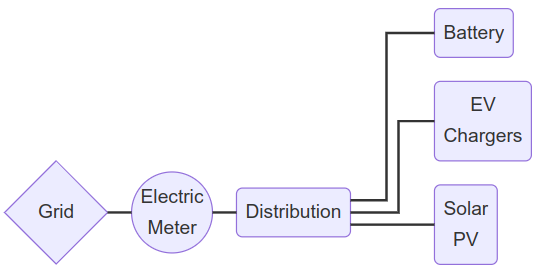
\includegraphics[width=7.5cm]{./images/oneline.png}
    \caption{Charging Site One Line Schematic. Simplified one-line schematic of the simulated EV charging station with true measured EV charging power, modeled on-site solar generation, and a modeled stationary battery for economic peak shaving.}
    \label{fig:oneline}
  \end{figure}

  \begin{equation}
    \label{eq:net-load}
    \begin{split}
      \exists B_d, B_c &\text{ s.t. } T \ge SL \forall t                                    \\      
             & \text{given:}                                                                        \\
      NL     & = L - S                                                                              \\
      SL     & = NL - B_d + B_c                                                                     \\
             & \text{where:}                                                                        \\
      t      & \in \mathbb{R}^+ [h] \text{ is the time step }      \\             
      NL(t)  & \in \mathbb{R} [kW] \text{ is the net load time series }                             \\
      L(t)   & \in \mathbb{R}^+ [kW] \text{ is the EV charging load time series }                   \\
      S(t)   & \in \mathbb{R}^+ [kW] \text{ is the solar production time series }                   \\
      SL(t)  & \in \mathbb{R} [kW] \text{ is the site load time series seen at the electric meter } \\
      B_c(t) & \in \mathbb{R}^+ [kW] \text{ is the battery charging load time series }              \\
      B_d(t) & \in \mathbb{R}^+ [kW] \text{ is the battery discharge time series }                  \\
      T(t)   & \in \mathbb{R}^+ [kW] \text{ is power threshold }                                    \\
    \end{split}
  \end{equation}

  The optimal threshold changes for each TOU period. A single simulation is defined for one solar configuration and battery capacity and lasts one calendar month, which is the shortest period for which the cost function is defined. Simulations are repeated for several months of data, and many different solar and battery design sizes, allowing for a retail energy cost comparison among different design scenarios. EV charging power and solar production are never curtailed. The primary decision variable in each time step is battery charge or discharge power, which is not necessarily formulated as a binary variable. Nonetheless, the battery can only charge, discharge, or do nothing in each time step.

  The main novelty of this work is studying the benefit of vertical bifacial PV modules in a peak shaving application, considering the sensitivity of the solution to a percentage of modules facing West and tilted vertically, battery capacity, and overall solar capacity.


  \subsection{Data}\label{data}%}

  %\subsubsection{{EV Charging Load }}\label{ev-charging-load}%}

  Measured EV charging power is used as the true load in the simulations and is never curtailed or rescheduled. For some sessions the EV charging time series was unavailable but the total charging energy was provided, in which case a constant charging power was assumed. The disaggregated session data is summed into a total site charging power time series, which is then downsampled to 15-minute intervals using the average value. Timestamp indices refer to the beginning of the 15-minute interval.


  %\subsubsection{Solar Production}\label{solar-production}%}

  Satellite irradiance data from the Geostationary Operational Environmental Satellite (GOES) is used as the primary data for modeling solar production and is obtained from the US National Solar Resource Database (NSRDB) \cite{Sengupta2018}. The data is serially complete and is available in 2 km by 2 km spatial resolution and 5-minute temporal resolution from 2018 onward. Multi-channel measurements from GOES are fed into the two-step Physical Solar Model (PSM) v3  \cite{Sengupta2018}. In the first step cloud and aerosol properties are collected and passed to the second step where the Fast All-sky Radiation Model for Solar Applications (FARMS), which estimates the radiation transfer on a tilted surface \cite{Xie2016}. Global Horizontal Irradiance (GHI) is computed directly from FARMS, then either REST2 or DISC models are used to compute Diffuse Normal Irradiance (DNI) if the environment is cloudy or clear, respectively \cite{Xie2018}. Authors indicate that computing surface irradiance in cloudy environments is complicated due to absorption and scattering within clouds, which may be a source of error relative to true measured solar PV production. Note these data are not organized into Typical meteorological Year (TMY) but are true satellite measurements for the same day and location as the EV charging load data.

  Solar DC power is modeled using the California Energy Commission Performance Model, a 6-parameter physical PV cell model The parameters are those for the Prism Solar 350 W bifacial solar module. The full AC array power is estimated given loss assumptions and an inverter efficiency lookup table specific to the Enphase IQH 380 W microinverter. All these functions are implemented in the US National Renewable Energy Laboratory (NREL) System Advisor Model (SAM) v2022.11.21 \cite{NREL2022}.

  %\hypertarget{battery}

  A stationary, storage, AC battery system is simulated as the only dispatchable asset in the peak shaving algorithm. In each time step the battery is chosen to charge or discharge within its technical limits. Because the control action is to hold the grid power exchange below a chosen threshold, batteries with a larger power capacity or energy capacity will necessarily achieve a lower threshold if the entire battery capacity is used. For a given energy capacity (\(kWh\)) those limits are a charge or discharge rate of no more than 1C and a state of charge (SOC) between 0 and 100\%. State of energy (SOE) is the SOC multiplied by nominal energy capacity and is reported in plots because the units are more meaningful when comparing dispatch time series. Half-round-trip charge and discharge efficiencies are constant at 90\%. Self-discharge and thermal limiting are not modeled specifically.

  There are many strategies for optimal battery sizing, but the emphasis in this work is instead on understanding the dynamics between load, the shape of the solar curve, and peak shaving algorithm for a given battery size. Therefore a sensitivity analysis is performed on the battery energy capacity, but no one battery size is declared economically optimal.

  Each simulation assumed charge and discharge rate are limited to 1C, usable SOC is assumed 100\%, and self-discharge, parasitic losses, and thermal limiting are not considered.

  \subsection{Electric Tariff}\label{electric-tariff}

  The total retail electric cost \(C\) for each month is then the sum of the energy cost and power cost for the month, where the energy and power costs are calculated separately for each TOU period. See Equation \ref{eq:cost}. The energy cost is the energy delivered to the site multiplied by the energy price for that TOU period. The power cost is the maximum of the 15-minute non-moving average load power for the month, multiplied by the power price for that TOU period. Only positive values of net load \(NL\) affect cost since the monthly peak power for each TOU period must always be positive and necessarily cannot benefit from net metering (export to the grid).

  \begin{equation}
    \label{eq:cost}
    \begin{split}
      C_m           & = \sum_k^K [p_{p,k,m}  max(SL^+_{k,m})] + \sum_k^K [p_{e,k,m} \sum (SL^+_{k,m}\Delta t) ]         \\
                    & \text{where:}                                                                             \\
      SL_{k,m}^+(t) & = SL(t) \forall SL(t)>0 \text{ in TOU period $k$ and month $m$}                           \\
      C_m           & \in \mathbb{R}^+ [\$] \text{ is total retail electric cost for month}\ m\                 \\
      p_{p,k,m}     & \in \mathbb{R}^+ [\$/kW] \text{ is power price for TOU period}\ k\ \text{and month}\ m\   \\
      p_{e,k,m}     & \in \mathbb{R}^+ [\$/kWh] \text{ is energy price for TOU period}\ k\ \text{and month}\ m\ \\
      K             & \in \mathbb{Z}^+ \text{ is the number of TOU periods} \\
      \Delta t      & = 0.25 [h] \\
    \end{split}
  \end{equation}

  Since the problem in question is economic peak shaving, the retail tariff is an important study parameter because it shapes the cost function and determines the benefit of solar production shifted into the late afternoon. With non-zero power prices, a threshold-based peak shaving approach is appropriate because it mimics the power component of the true cost function, which concerns the maximum value and not every individual power value. Once the threshold is met, the optimizer knows that "power is free" and will charge the battery up the threshold without penalty to the cost function. Energy of course is paid by the integral of power and therefore any marginal consumption results in a marginal cost.

  %\hypertarget{peak-shaving-algorithm}

  An optimal peak shaving strategy is used to minimize the total retail electric cost to the EV charging station. The strategy is operational only and assumes the solar production time series and battery capacity are fixed. The state variable controlled by the algorithm is battery charge or discharge power. However, the algorithm reframes the problem as one of choosing a power threshold \(T\ [kW]\) applied to the point of injection to the grid, the electric meter. The battery is then dispatched, within its technical limits, to hold the net load ($L-S$) below the threshold. When the algorithm is successful the different thresholds for each TOU period are met for an entire month. If the battery reaches a technical limit and net load exceeds a threshold, the simulation is not necessarily invalid but is not likely to minimize the retail electric cost to the site for that combination of solar and battery size. The peak shaving logic is described in Figure \ref{fig:peakshaving-flowchart}.

\begin{figure}
  \centering
  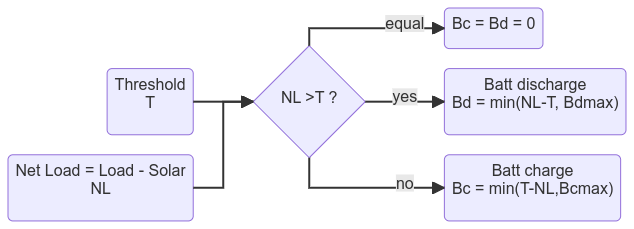
\includegraphics[width=7.5cm]{./images/peak shaving flowchart.png}
  \caption{Peak Shaving Flowchart. Net load is the time series of load with solar subtracted. There is one threshold value for one for each TOU period with a non-zero power price. For each timestep of the simulation, the net load is compared to the threshold of the current TOU period. The battery is discharged if the net load is greater than the threshold and charged if the net load is less than the threshold. If the two are equal or if there is no power price the battery does nothing.}
  \label{fig:peakshaving-flowchart}
\end{figure}

The peak shaving algorithm describes stepping through time and dispatching the battery according to given power thresholds, which are chosen separately by an optimizer.

%\hypertarget{threshold-optimizer}

The optimal demand thresholds (one per TOU period) are determined by a custom gradient descent optimizer based on the Newton-Raphson method \cite{Truong2019}. The objective function \(C\) minimizes the retail energy cost of one month, which is the billing interval of this retail electric tariff. See Equation \ref{eq:optimization}. In practice, the optimal thresholds are different for each month. The threshold for each TOU period \(T_k\) is not enforced to be non-negative, but in practice always is because the cost function \(C_m()\) cannot evaluate to a negative value.

\begin{equation}
  \label{eq:optimization}
  \begin{split}
    min[C_m(B_c,B_d)] & = min[C_m(T_1,T_2,..T_K)]                                                                          \\
                      & s.t.                                                                                               \\
    B_c(t)            & \le B_{c,max}                                                                                      \\
    B_d(t)            & \le B_{d,max}                                                                                      \\
    SOC_{min}         & \le SOC \le SOC_{max}                                                                              \\
                      & \text{where:}                                                                                      \\
    T_k               & \in \mathbb{R}^+ [kW] \text{ is threshold for}\ k\text{-th TOU period of}\ K\ \text{total periods} \\
    SOC(t)            & \in \mathbb{R}^+ \le 1 [kWh/kWh]  \text{ is battery state of charge timeseries}\                   \\
  \end{split}
\end{equation}

Beginning from an initial guess the Newton-Raphson gradient descent optimizer calculates the batch gradient and updates parameters based on a learning rate of 0.01 \cite{Truong2019}. This continues until the stopping condition is met, minimum cost for a patience of 50 iterations. The Newton-Raphson gradient descent-based optimization method is preferred over linear programming because it will minimize a variety of cost functions without needing to reformulate the linear program for each case.

%\hypertarget{simulations}

Simulations are run one month at a time for a given solar array orientation and battery capacity, according to the flowchart in Figure \ref{fig:simulation-flowchart}. The threshold optimizer produces one threshold value (kW) for each TOU period with non-zero power prices. This returns both optimal thresholds and a minimum cost. Finally, a 1-month simulation of the battery charging and discharging is performed to ensure no violations of the battery technical limits and to produce the battery power time series for evaluation. The computational environment is Python 3.8 in Windows 10 64-bit, on an Intel i9 CPU with 64 GB of RAM.

\begin{figure}
  \centering
  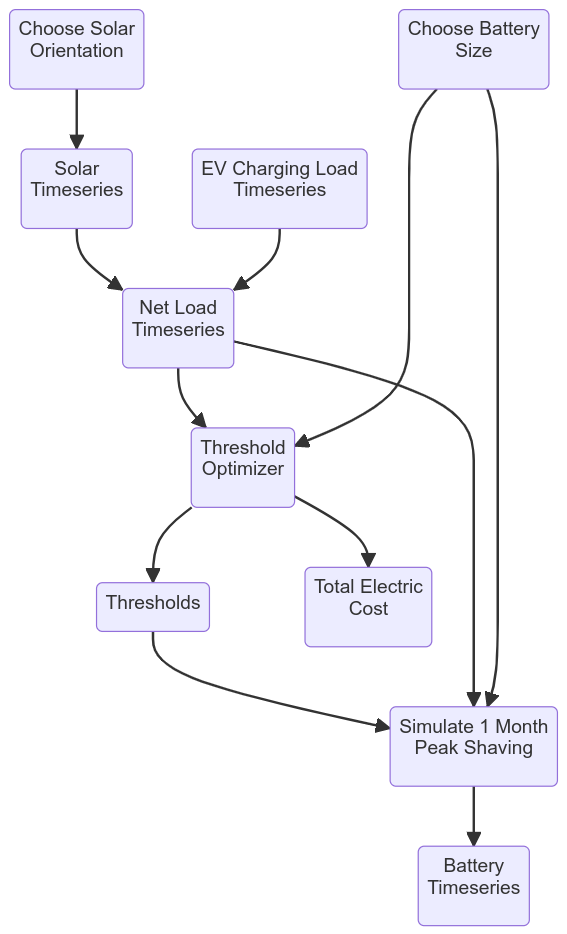
\includegraphics[width=\linewidth]{./images/simulation flowchart.png}
  \caption{Simulation Flowchart. For each solar array case, battery capacity, and set of power thresholds, a single simulation is performed on the data 1 month at a time.}
  \label{fig:simulation-flowchart}
\end{figure}

%\hypertarget{case-studies}

All case studies use the same electric load and tariff, and solar production changes for each case. The load is measured EV charging power ("load") from the Caltech Adaptive Charging Network database at the Jet Propulsion Lab (JPL) site \cite{Lee2021}. The time series data interval is 10 s, and the data period is from 2018-5-1 00:00 to 2019-2-28 23:45. See Table \ref{tab:data-summary}. The electric tariff is typical for California and consists of several different TOU periods, summarized in Table \ref{tab:tariff}. Each TOU period may have an energy price (\(\$/kWh\)), a power price (\(\$/kW\)), or both. Some prices change seasonally as well.

% The two largest power prices are 26.07 $\$/kW$ associated with the "All hours" period for all seasons and 32.90 $\$/kW$ associated with the "Peak (Summer)" period of 16:00-21:00, when the vertical West-facing bifacial modules will produce more energy in the late afternoon and evening than the South-facing modules. Since load curtailment is not considered, the battery will only have the option to shift energy from the expensive Peak period to other periods. Since all other periods have the 26.07 $\$/kW$ price, the marginal power cost reduction for shifting 1 kW of peak load out of the Peak period is only \$32.90.  

\begin{table}[!h]
  \centering
  \caption{Timeseries Data Summary. The primary data sources are Caltech ACN EV charging power and GOES solar irradiance. Solar production is modeled from irradiance.}
  \label{tab:data-summary}
  \begin{tabularx}{\linewidth}{XXXXX}
    \toprule
    Description                     & Location                                & Type                                                                                                                  & Interval                               & Source                                \\
    \midrule
    EV charging power $[kW_{ac}]$   & Jet Propulsion Lab, Pasadena CA, USA    & Measured and aggregated from multiple  EV chargers at single site                                                     & 10 sec (average downsampled to 15 min) & Caltech ACN (site JPL) \cite{Lee2021} \\
    Solar irradiance $[W/m^2]$      & GPS: 34.2013, -118.1721 (2x2 km square) & GOES satellite irradiance                                                                                             & 5 min                                  & NSRDB PSMv3 \cite{Sengupta2018}       \\
    PV array production $[kW_{ac}]$ & GPS: 34.2013, -118.1721 (2x2 km square) & Modelled from GOES satellite irradiance, 368 Prism Solar 350 W bifacial modules, 368 Enphase IQH 380 W microinverters & 15 min                                 & SAM \cite{NREL2022}                   \\
    \bottomrule
  \end{tabularx}
\end{table}

\begin{table}[!h]
  \centering
  \caption{Retail Electric Tariff. An applicable electric tariff schedule with power and energy prices for several different TOU periods. From California PG\&E.}
  \label{tab:tariff}
  \begin{tabularx}{\textwidth}{XXXXX}
    \toprule
    Name            & TOU Period                         & Summer (Jun 1 - Sept 30) $[\$]$ & Winter (Oct 1 -Feb 28) $[\$]$ & Spring (Mar 1 - May 30) $[\$]$ \\
    \midrule
    All hours       & 0:00-0:00     3                    & 26.07/$kW$                      & 26.07/$kW$                    & 26.07/$kW$                     \\
    Super off-peak  & 9:00-14:00                         & -\/-                            & -\/-                          & 0.079/$kWh$                    \\
    Off-peak spring & 0:00-9:00, 14:00-16:00, 21:00-0:00 & -\/-                            & -\/-                          & 0.132/$kWh$                    \\
    Off-peak winter & 0:00-16:00, 21:00-0:00             & -\/-                            & 0.132/$kWh$                   & -\/-                           \\
    Off-peak summer & 0:00-14:00, 23:00-0:00             & 0.132/$kWh$                     & -\/-                          & -\/-                           \\
    Partial-peak    & 14:00-16:00, 21:00-23:00           & 6.81/$kW$, 0.159/$kWh$          & -\/-                          & -\/-                           \\
    Peak            & 16:00-21:00                        & 32.90/$kW$, 0.196/$kWh$         & 2.22/$kW$, 0.172/$kWh$        & 2.22/$kW$, 0.172/$kWh$         \\
    \bottomrule
  \end{tabularx}
\end{table}

The five case studies in Table \ref{tab:casestudies} consider different solar orientations, each with an increasing percentage of the modules oriented West and tilted vertically. The solar production time series for all cases is modeled in SAM from GOES satellite irradiance (Table \ref{tab:data-summary}), with one Enphase IQH 380 W microinverter per Prism 350 W bifacial solar PV module, for 368 microinverters and 368 PV modules total.

The base case is a typical South-facing array tilted at 20˚, called South 20˚ in Table \ref{tab:casestudies}. This is intended to be a compromise between the high tilt angles suggested in \cite{Baghoolizadeh2022} and the low rooftop tilt angles preferred by industry for the higher coverage ratio and lower wind load \cite{Cao2013}. The daily clear sky solar power profile is the familiar rounded triangle centered at solar noon, such as in Figure \ref{fig:weekly-load-solar}. The array is sized such that the total energy produced is equal to the total energy consumption of the EV charging station. This "net zero" sizing is not necessarily economically optimal, but rather it is a reasonable assumption for a solar capacity given the load.

The remaining four case studies in Table \ref{tab:casestudies} consider a percentage of the array permanently rotated West and tilted 90°: 25\%, 50\%, 75\%, and 100\%. The last case is extreme from a design perspective but should be investigated since it represents a maximum amount that midday production can be time-shifted into the late afternoon and evening without tracking or storage. Graphically that shift results from the M-shaped daily power profile seen in Figure \ref{fig:weekly-load-solar}. Microinverters are used in the design so that the cases with a percentage of the array facing West can are indeed a linear combination of the M-shaped and rounded-triangle power profiles.

\begin{table}
  \centering
  \caption{Case Studies. All modules are the Prism 350 W bifacial. The base case array faces South and is tilted to 20°. The following four cases orient an increasing percentage of the modules West and tilt to 90°, with an expected linear decrease in total energy and solar yield.}
  \label{tab:casestudies}
  \begin{tabularx}{\textwidth}{XXXXXX}
    \toprule
    Case Study                     & Modules & Orientation & Tilt & Total Energy ($MWh$)   & Solar Yield ($\frac{kWh}{kW_{DC}}$) \\
    \midrule
    South 20° (base)               & 368     & South       & 20°  & 151.7                  & 1180.8                              \\
    \hline
    \multirow{2}{*}{25\% West 90°} & 276     & South       & 20°  & \multirow{2}{*}{146.5} & \multirow{2}{*}{1140.4}             \\
                                   & 92      & West        & 90°  &                        &                                     \\
    \hline
    \multirow{2}{*}{50\% West 90°} & 184     & South       & 20°  & \multirow{2}{*}{141.1} & \multirow{2}{*}{1098.2}             \\
                                   & 184     & West        & 90°  &                        &                                     \\
    \hline
    \multirow{2}{*}{75\% West 90°} & 92      & South       & 20°  & \multirow{2}{*}{136.1} & \multirow{2}{*}{1059.6}             \\
                                   & 276     & West        & 90°  &                        &                                     \\
    \hline
    100\% West 90°                 & 368     & West        & 90°  & 131.0                  & 1019.3                              \\
    \bottomrule
  \end{tabularx}
\end{table}

%\hypertarget{results}

The peak shaving methodology produces an optimally low retail electric cost for each of the 10 months of data, which are summed up for total electric cost versus the battery capacity sensitivity analysis. See Figure \ref{fig:total-cost}. The costs monotonically decrease with battery capacity as expected because every marginal unit of added battery energy capacity allows the algorithm to hold a power threshold for longer, and since each battery is rated for 1C at charging and discharging, the battery will also have more power capacity to achieve lower thresholds relative to the same size peak. The 100\% West 90° array achieves a lower total cost than the baseline South 20°. All three combination arrays achieve a lower cost for all battery capacities up to 200 kWh, with a maximum reduction of \$1422 (6.7\%) relative to the South 20° with a 100 kWh battery. The largest percentage improvement of 7.10\% (\$1208) occurs for the same array but 150 kWh battery. The absolute cost reduction is likely more important than the relative reduction since it would be treated directly as revenue in a cash flow analysis to determine the economic performance of a given battery.

\begin{figure}[!h]
  \centering
  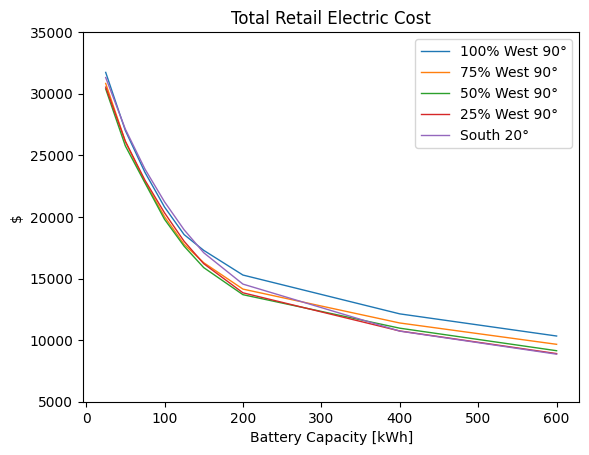
\includegraphics[width=0.49\textwidth]{./images/total cost.png}
  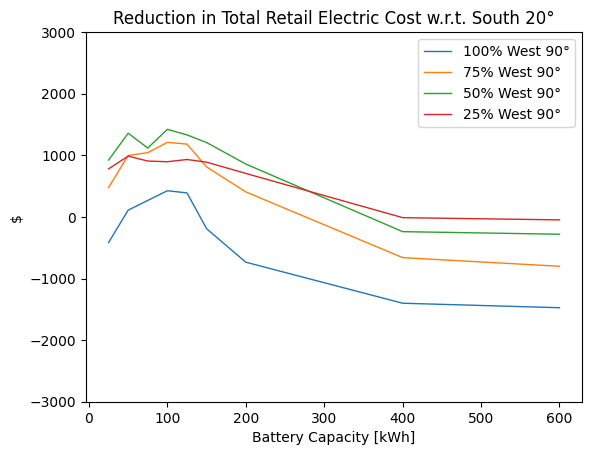
\includegraphics[width=0.49\textwidth]{./images/total cost reduction.png}
  \caption{Total Retail Electric Cost. Costs are calculated for each case study and a sensitivity analysis is performed on battery capacity (kWh). Below 150 kW the South 20° and 100\% West 90° arrays have similarly high total costs, whereas the three combination arrays are somewhat grouped a few percent below. Above 150 kW the total costs for each case diverge somewhat, with the South 20° base case attaining the lowest cost for the 400 kWh battery and larger. RIGHT: Reduction in Total Retail Cost is likely the most important metric for evaluating the peak shaving efficacy since it can be directly used as revenue in a cash flow analysis to calculate economic performance. The combination of the 50\% West 90° array and 100 kWh battery achieved the largest cost reduction of \$1422 (6.7\%) over the 10-month data period. A selection of the data generating these graphs is shown in Table \ref{tab:data-summary}.}
  \label{fig:total-cost}
\end{figure}

The benefit of vertical bifacial modules can be seen when comparing the simulated battery charge and discharge time series data. Figure \ref{fig:peak-shaving} shows the same day (June 6) for both the base Solar 20° case and the 100\% West 90° case, which is presented here as a clearer graphical example than the better-performing 50\% West 90° array. For both cases, June 6 is the limiting day for the month, when the battery reaches a technical limit, in these cases zero SOC. This is likely due to a particularly large evening peak load event from approximately 17:30 to 21:30, with a maximum power of 56 kW and total energy of 201 kW. For these simulations, the battery capacity is 125 kWh nominal and 112.5 kWh after losses, and as specified the battery will charge and discharge at a maximum of 1C or 125 kW. In Figure \ref{fig:peak-shaving} the base case of South 20° overproduces in the middle hours of the day and solar is exported to the network starting around 12:00. During the peak load event the South 20° only produces 18.8 kWh whereas the 100\% West 90° array produces 104 kWh. In each case the battery charges to 100\% (125 kWh) before the evening peak load event. The result is that the evening net load peak in the 100\% West 90° case starts later and contains less energy, though it reaches the same maximum power. Due to this the battery in the 100\% West 90° case can hold the site load to a lower threshold in \(kW\), which is directly proportional to reducing the retail electric cost. During the expensive "Peak" TOU period of 14:00-21:00, the base South 20° case only achieves a low threshold of 13.0 kW, whereas the 100\% West 90° case holds a threshold of 3.1 kW in the same period, a 76\% improvement. The retail electric cost isn't defined for only one day out of a typical month, since the power portion of the cost is calculated on the monthly peak. However if June 6 was the only day of the month with non-zero load the total cost would be \$983 for the South 20° case and \$560 for the 50\% West 90° case, which is a 43\% reduction.

\begin{figure}[!h]
  \centering
  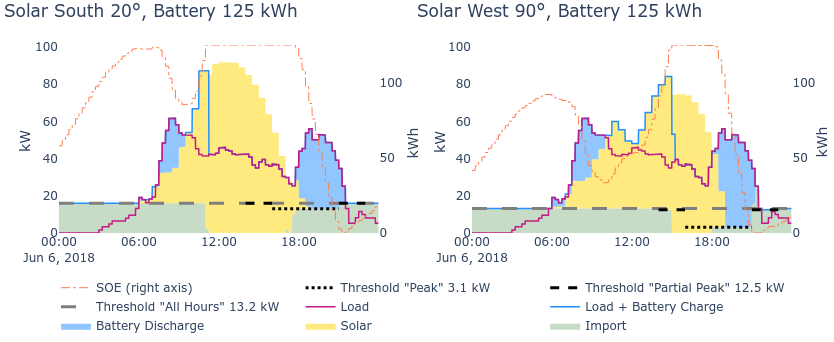
\includegraphics[width=\textwidth]{./images/single day of peak shaving.png}
  %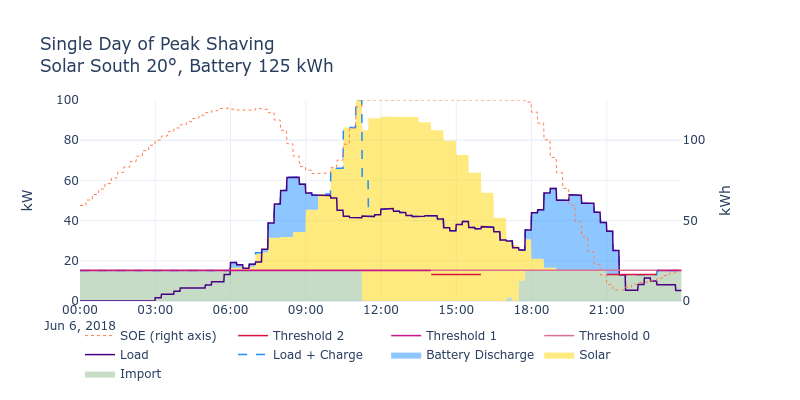
\includegraphics[width=6.8cm]{./images/single day of peak shaving south.png}
  %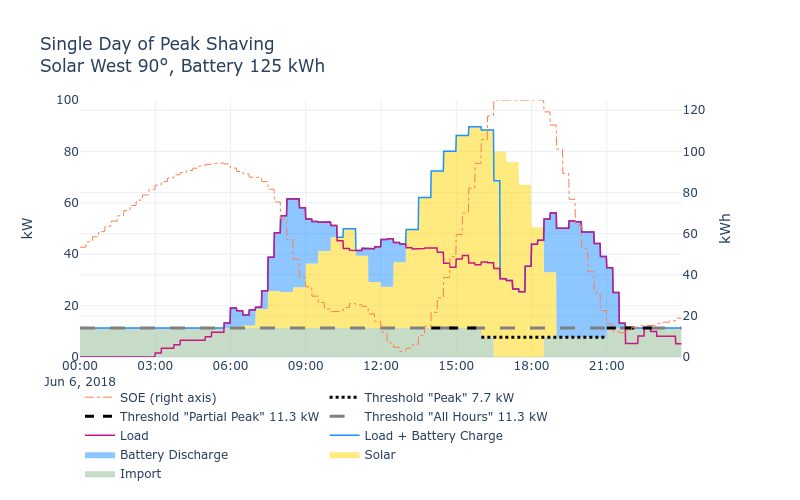
\includegraphics[width=6.8cm]{./images/single day of peak shaving west.png}
  \caption{Single Day of Simulated Peak Shaving. Solid lines are load from EV charging (magenta) and the additional amount of storage battery charging (blue). Solid areas are energy sources and always sum up to the load unless solar production is greater than the load and is exported to the grid. Dashed line segments are TOU power thresholds. The dash-dot line is SOE, referenced to the right vertical axis. LEFT: The base South 20° solar array overproduces midday and exports energy to the grid. RIGHT: The 100\% West 90° case shifts production to the late afternoon, reducing the evening load energy and thereby the Peak period threshold to 7.7 kW, 42\% lower than the South 20° array.}
  \label{fig:peak-shaving}
\end{figure}

In Table \ref{tab:total-cost} are some of the data from Figure \ref{fig:total-cost}, though not shown for conciseness are the 75\% West 90° and the 25\% West 90° cases. The largest cost reduction is \$1422 for the 50\% West 90° case and 100 kWh battery. Note that the largest reduction in retail cost may not be the best solution economically, since the 25 kWh battery achieves 65\% of the cost reduction at 20\% of the battery energy capacity, which is roughly proportional to capital cost.

\begin{table}[!h]
  \centering
  \caption{Total Retail Electric Cost. Simulated total retail electric cost for three of the case studies (some omitted for conciseness) over the 10 months of available data and a given battery capacity. Cost reduction is calculated with respect to the South 20° base case. The best reduction in total retail cost is \$1422 for the 50\% West 90° case.}
  \label{tab:total-cost}
  \begin{tabularx}{\textwidth}{XXXXXXXX}
    \toprule
    Battery $[kWh]$ & \multicolumn{3}{l}{Cost $[\$]$} & \multicolumn{2}{l}{Cost Reduction $[\$]$} & \multicolumn{2}{l}{Cost Reduction $[\%]$}                                                                   \\
                    & South 20°                       & 50\% West 90°                             & 100\% West 90°                            & 50\% West 90° & 100\% West 90° & 50\% West 90° & 100\% West 90° \\
    \midrule
    25              & 31314                           & 30391                                     & 31730                                     & 923           & -416           & 3.0           & -1.3           \\
    50              & 27132                           & 25773                                     & 27022                                     & 1359          & 110            & 5.0           & 0.4            \\
    75              & 23893                           & 22775                                     & 23625                                     & 1118          & 268            & 4.7           & 1.1            \\
    100             & 21229                           & 19807                                     & 20804                                     & \textbf{1422} & 425            & 6.7           & 2.0            \\
    125             & 18954                           & 17623                                     & 18564                                     & 1331          & 390            & 7.0           & 2.1            \\
    150             & 17094                           & 15886                                     & 17286                                     & 1208          & -192           & 7.1           & -1.1           \\
    200             & 14547                           & 13689                                     & 15282                                     & 858           & -735           & 5.9           & -5.0           \\
    400             & 10730                           & 10969                                     & 12131                                     & -239          & -1401          & -2.2          & -13.1          \\
    600             & 8859                            & 9140                                      & 10333                                     & -281          & -1474          & -3.2          & -16.6          \\
    \bottomrule
  \end{tabularx}
\end{table}

A sensitivity analysis on the size of the solar array is performed with the results in Figure \ref{fig:solar-sensitivity} and Table \ref{tab:solar-sensitivity}. The total retail cost decreases monotonically with the larger solar capacities and the cost reduction increases by a factor of 10 from the smallest to largest solar capacity. This result is expected since the larger capacities create a more pronounced difference between the late afternoon production of the two arrays and the peak shaving strategy translates into lower power thresholds for the cases with some portion of the array in the 100\% West 90° orientation. The 50\% West 90° case performs best in the first four solar capacities at which point, for the first time, the best performing case is one where the majority of the modules are in the 100\% West 90° orientation (75\%). However, the difference of \$19 is not substantial. At larger solar capacities the cost reductions for each case study are both larger in magnitude and closer together, however, the increase in cost reduction is clearly less than linear with solar capacity. This suggests a diminishing returns problem where, after a certain capacity of 100\% West 90° modules is met, the additional South 20° and 100\% West 90° modules are providing energy when the battery is already at 100\% SOC.


\begin{table}[!h]
  \centering
  \caption{Solar capacity sensitivity analysis based on reduction in total retail cost relative to the base South 20° case. While the 50\% West 90° array continues to achieve the highest cost reduction, the battery capacity increases from 25 kWh to 125 kWh.}
  \label{tab:solar-sensitivity}
  \begin{tabularx}{\textwidth}{XXXX}
    \toprule
    Solar Capacity {[}\(kW_{DC}\){]} & Best Case for Cost Reduction         & Best
    Cost Reduction {[}\${]}          & Best Cost Reduction Battery Capacity
    {[}kWh{]}                                                                            \\
    \midrule
    64.4 (0.5x)                      & 50\% West 90°                        & 260  & 25  \\
    128.8 (1.0x)                     & 50\% West 90°                        & 1422 & 100 \\
    193.2 (1.5x)                     & 50\% West 90°                        & 2211 & 125 \\
    257.6 (2.0x)                     & 75\% West 90°                        & 2579 & 125 \\
    \bottomrule
  \end{tabularx}
\end{table}


\begin{figure}
  \centering
  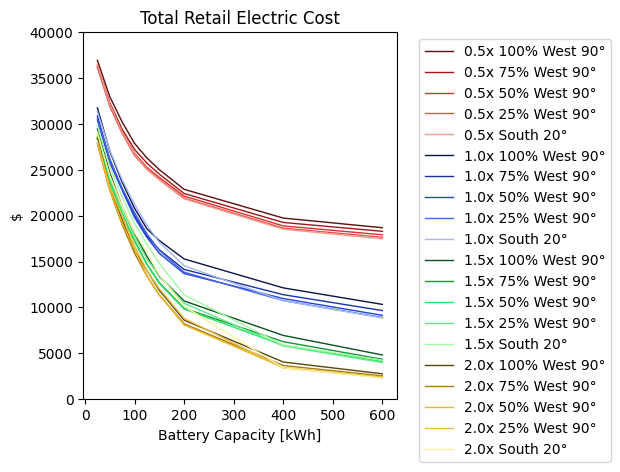
\includegraphics[width=0.8\linewidth]{./images/total cost reduction solar sensitivity.png}
  \caption{Solar Capacity Sensitivity. A sensitivity analysis on solar capacity shows more available cost reduction, which increases less than linearly with solar capacity.}
  \label{fig:solar-sensitivity}
\end{figure}

The battery capacities increase from 25 kWh up to 125 kWh across the solar sizes, which is an unexpected finding. Despite the extra capacity the 100\% West 90° case in Figure \ref{fig:weekly-load-solar} is still mostly unable to affect the peak power of the evening peaks, and thus both the base South 20° and combination array cases have a similar maximum power to shave. Indeed the average of the monthly peak net load values is 74.5 kW for the South 20° 2.0x case and 74.7 kW for the 100\% West 90° 2.0x case. However, when increasing the solar to 2.0x, the energy under the net load time series during the 17:00 to 22:00 period decreases by only 164 kWh for the South 20° versus 886 kWh for the 100\% West 90° case. With more solar production in the evening peak, the optimizer is able to pursue driving the "Peak" TOU period to zero, which has a large economic benefit. This is unachievable with the small battery capacities and is more difficult without the late afternoon solar production of the 100\% West 90° modules. Indeed a large 200 kWh battery is required to achieve the first 0 kW "Peak" period threshold in the South 20° case for all solar capacities. Rather, the 100\% West 90° case achieves a 0 kW Peak period threshold with the 150 kWh battery at 100\% solar capacity and with the 125 kWh battery at 2.0x solar capacity.

\begin{figure}
  \centering
  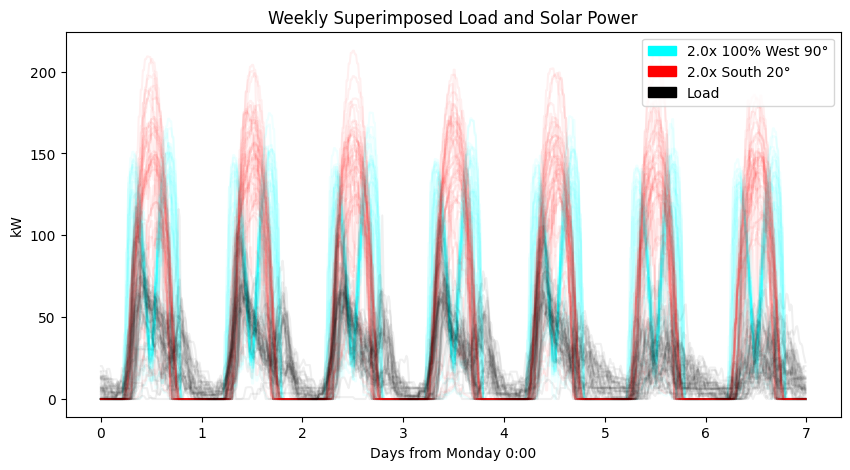
\includegraphics[width=\linewidth]{./images/weekly load solar.png}
  \caption{Weekly Overlaid Load and Solar Power. The entire 10-month time series of EV charging load, Solar 20°, and 100\% West 90° are superimposed on a weekly basis, beginning on Monday. The 100\% West 90° case provides a clearer graphical example than the better-performing cases.}
  \label{fig:weekly-load-solar}
\end{figure}

%\hypertarget{conclusion}

An optimal electric load peak shaving strategy is simulated on 10 months of EV charging power time series. The peak shaving asset is a storage battery with a maximum charge and discharge rate of 1C and a constant discharge and charge efficiency of 90\%. A co-located solar array is included in the simulation to study the effects of typical South-facing modules vs. West-facing vertical bifacial modules. Five different array orientations are presented as different case studies. In addition, sensitivity analyses on battery energy capacity and solar array capacity provide information about the dynamics of the optimal peak shaving algorithm. The best-performing case is designed with 50\% of the array South facing tilted at 20° and 50\% facing West at 90°, which achieved a reduction in the total retail cost of energy of \$1422 (6.7\%) with a 25 kWh battery. The cost reduction is relative to the base case array with all the modules facing South and tilted at 20°. When solar is increased to twice the net-zero capacity the best-performing case is 75\% West 90° with a cost reduction of \$2579 (16.1\%) with a 125 kWh battery. The best percentage cost reduction overall is 20.0\%. Both data and code are shared with the public on GitHub.

Peak shaving a monthly peak power typically, depending on the load factor, results in dispatching the battery until its technical limits to achieve a minimum monthly peak power. Because the load, or net load after solar is dispatched, is often not very homogeneous there will be one limiting day where the battery is bound by its technical limits and the peak power of the month is set. The presence of this limiting day in the month simulation of Figure \ref{fig:peak-shaving} does not guarantee a global minimum cost, but the lack of a limiting day would suggest the global minimum was not found. Intuitively the limiting day can be thought of as the most difficult day for the battery to achieve the given thresholds, and if the day was somehow easier for the battery (less and more uniform net load) the power thresholds could be lowered and therefore a lower retail electric cost achieved. Because the results of each month typically depend strongly on one limiting day, small changes in the load or the solar power magnitude or temporal relationship can have a large impact on the overall results. For this reason, peak shaving simulations require particular care in data selection, cleaning, and acquiring an appropriately large amount of data such that the probability space of true possible limiting is well represented in the selected sample of limited days.

Confidence in the results presented is medium-high given the use of true EV charging measurements, a robust Newton-Raphson gradient descent optimizer with verified optimality, a true electric tariff appropriate for the load site and solar data location, and sensitivity analyses performed on two variables. Future work should include more load data sets with more months of data, a more comprehensive battery model, an operational peak shaving strategy based on a load forecast, and testing at the Politecnico di Milano M2GLab microgrid.

%\hypertarget{bibliography}

\bibliography{mendeley.bib}

\end{document}
